\section{Contesto e Finalità}
Per comprendere nella sua complessità un progetto di questo tipo, è necessario tenere conto prima di tutto del contesto in cui viene sviluppato e delle finalità implicite ed esplicite che si vogliono raggiungere.
Nel caso di questo elaborato si tratta, prima di tutto, di descrivere lo sviluppo di un applicativo mobile fortemente legato ai sistemi di marketing e alle nuove strategie di business di aziende leader all'interno dei propri mercati, in molti casi saturi o fortemente instabili, scossi dalle innovazioni tecnologiche di questi decenni.

Oltre alle ingerenze esterne sul progetto, come il cambiamento repentino delle tecnologie o la presenza di eventuali competitor, deve essere valutata la posizione del singolo componente all'interno dello sviluppo dell'interno progetto, la quale va tenuta in forte considerazione specialmente durante la prima fase di sviluppo in cui si determinano le prime linee guida da seguire durante tutto il lavoro.

Questo elaborato rientra nel concetto di \textit{Application Economy}, che descrive perfettamente il trend degli ultimi anni: il cambiamento dei metodi con cui le masse ottengono informazioni e si lasciano influenzare hanno portato ad un sostanziale sconvolgimento del sistema di marketing e delle strategie commerciali anche di aziende multinazionali. 
Proprio in questo contesto è necessario inquadrare le motivazioni che hanno portato l'azienda Carpigiani a dare vita all'ecosistema MyGelato, di cui questa tesi sviluppa solo una componente, così da realizzare quanto progetti di questo tipo siano fondamentali in questo momento storico.
Si tratta di uno studio in ambito pubblicitario, che ha finalità implicite legate fortemente all'ambito commerciale e produttivo dell'azienda.


\subsection{Application Economy}
  
\begin{figure}[h!]
  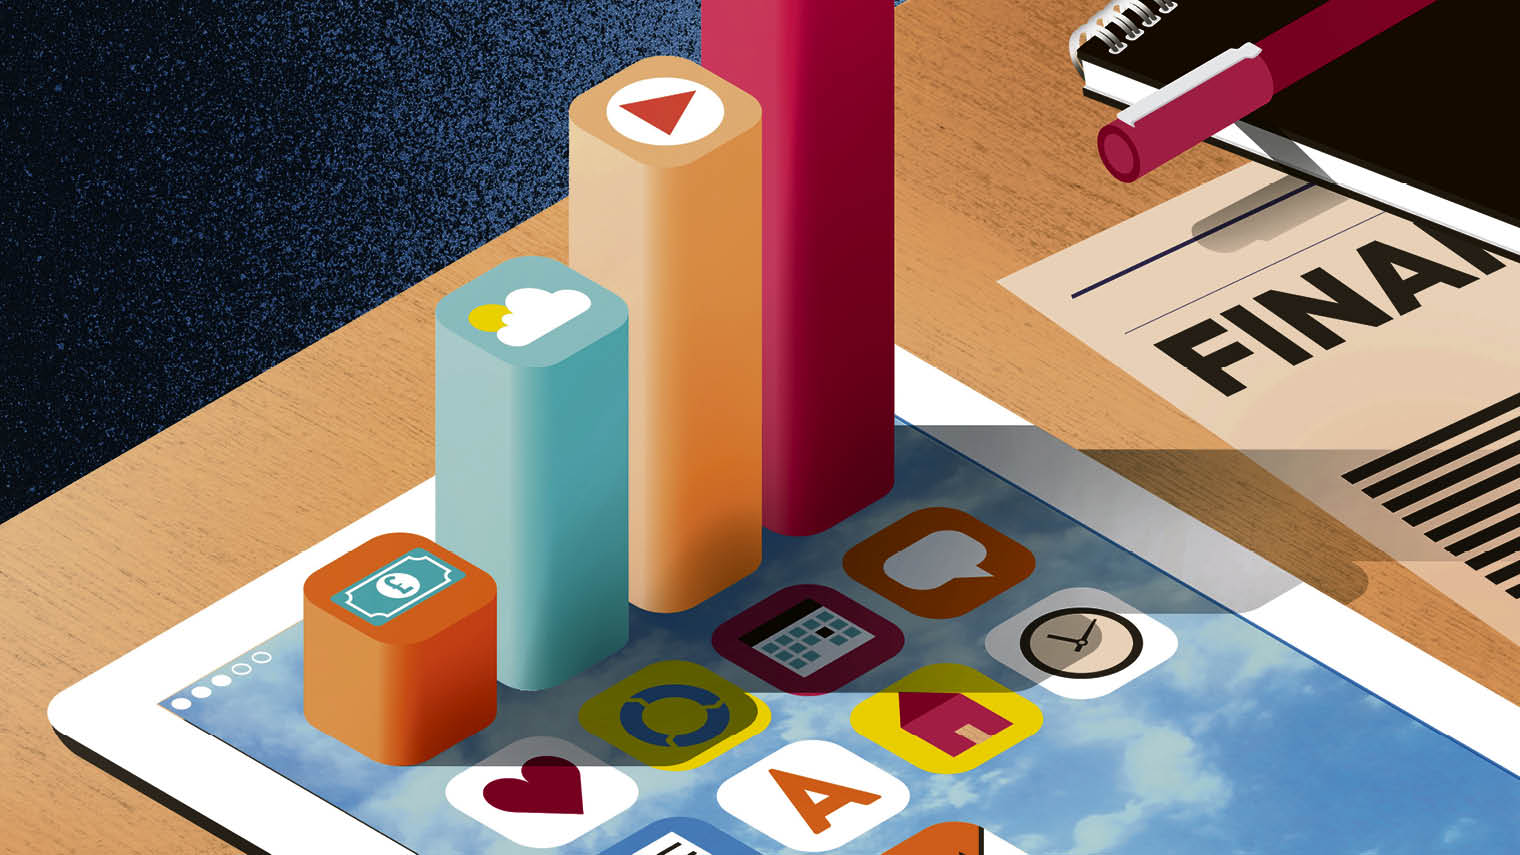
\includegraphics[width=\linewidth]{images/The-App-Economy.jpg}
  \caption{Applications Economy}
  \label{fig:appEconomy1}
\end{figure}
  
Non vi è forse modo di descrivere la società attuale e questo periodo storico senza valutare l'importanza dello sviluppo tecnologico che ci ha portato in quella che viene definita l'\textit{Era dell'Informazione}.
La rivoluzione tecnologica che sta avvenendo in questi anni, specialmente a partire dagli anni Novanta, ha portato la connessione globale a internet ad assumere un ruolo essenziale in ogni aspetto della società moderna e della nostra vita.

È cambiato drasticamente il modo con cui le persone accedono alle informazioni, che siano queste di tipo personale o di tipo commerciale.
Allo stesso modo si sono dovute adeguare le strategie di tutte quelle aziende che hanno visto cambiare in maniera drastica il proprio mercato, invaso molte volte da tecnologie sempre diversificate e innovative.

Secondo il giornalista Paul Mason, è stata la dottrina economica degli ultimi decenni della nostra epoca che da una parte ha avuto il merito di promuovere la più grande ondata di sviluppo economico che il mondo abbia mai visto, ma dall’altra ha portato a mercati incontrollati e a vorticosi cambiamenti sociali innescati dalla tecnologia.
Si sono diffusi, infatti, concetti come i progetti open-source, la sharing economy e le licenze creative commons che hanno messo in crisi le fondamenta del capitalismo odierno: la proprietà privata. 
Questo fenomeno unito alla saturazione di molti mercati ha portando tante aziende a dover rivedere la propria business strategy obbligandole a dirigere i propri investimenti sulla diversificazione e sulle nuove strategie di vendita. \autocite{POSTCAPITALISMO}

Prime su tutte sono diventati di fondamentale importanza l'e-commerce e il marketing digitale, fortemente spinti dalle tecnologie e dalla nuova possibilità di accedere a una risorsa comune (Internet) da parte della maggior parte della persone anche di cultura, età e ambienti sociali diversi.
Legato alla diffusione sempre crescente di smartphone, nasce quindi l'Application Economy: lo sviluppo e l'utilizzo di applicazioni mobile per raggiungere gli utenti consumatori.
Questa strategia può essere applicata, per esempio, in ambito marketing per pubblicizzare un proprio prodotto, fidelizzare il consumatore alla propria azienda e mantenere una propria immagine in un sistema in cui l'idea che i consumatori hanno dell'azienda è fondamentale.

Forse ancora in via di sviluppo per certi settori ma ormai sempre più diffuso, è l'e-commerce, la possibilità di fare acquisti online, che sta spostando il modo di comprare online sempre più sui device mobile (una statistica del BI Intelligence riporta che entro il 2020 il commercio mobile supererà il 45\% degli acquisti online complessivi).
Questa soluzione permette all'utente di pagare direttamente tramite sistemi bancari e non più tramite contanti, spostando inoltre il controllo delle vendite dal rivenditore al fornitore di servizi.

\subsection{Ecosistema MyGelato}

L'ecosistema MyGelato si pone proprio all'interno di questo contesto, ad unire le strategie di marketing dell'azienda produttrice Carpigiani e delle singole gelaterie convenzionate; insieme alla possibilità di comprare, regalare e utilizzare online dei coupons che permettono l'acquisto di gelati.

È un progetto di piattaforma web e mobile che si rivolge al pubblico dei gelatieri e dei consumatori di gelato. Gli obiettivi commerciali sono diversi, primi tra i quali quello di incentivare la compravendita di gelati tramite il sistema di coupons digitali e quello di promuovere il consumo di gelato tramite offerte, fornendo anche ai gelatieri un sistema semplice ed efficace per pubblicizzare il proprio negozio.

Attraverso l'applicativo, l'utente può informarsi sulle gelaterie presenti in zona verificando anche quali facciano parte del circuito MyGelato.
È possibile selezionare ogni gelateria così da avere alcune informazioni utili, come indirizzo e numero di telefono, salvarle nei preferiti e verificare se vi sono promozioni attive.
Nel momento in cui l'utente aggiunge ai preferiti una gelateria, verrà informato tramite notifica push di eventuali nuove promozioni attive e sarà notificato l'essere arrivato vicino ad una gelateria di proprio interesse.
Queste strategie sono ovviamente di carattere pubblicitario e permettono anche a gelaterie minori, facenti però parte del circuito, di essere pubblicizzate dagli utenti che utilizzano la piattaforma.

Questo sistema permette all'azienda Carpigiani di avere un controllo maggiore su un sistema centralizzato di advertasing per le gelaterie di cui è principale fornitore, ottenendo quindi la possibilità di intervenire su realtà locali standardizzandone alcuni meccanismi.

Seconda feature fondamentale dell'applicazione, che riguarda in questo caso solo gli utenti iscritti al sistema, è la possibilità di comprare online dei coupon digitali che permetto l'acquisto, tramite bruciatura, di un gelato di una determinata gelateria.
Questi coupon sono visualizzabili in ogni momento e possono essere regalati anche ad altri utenti tramite un semplice metodo di condivisione/riscatto che permette al destinatario di usufruire dell'oggetto comprato.
Ogni gelateria che supporta questo sistema sarà provvista della stessa applicazione con un account gelatiere che permetterà di bruciare i coupon utilizzati, per i quali verrà in seguito rimborsata direttamente dall'azienda.

Questo sistema di e-commerce sposta la vendita di un prodotto molto semplice come i gelati, online; È infatti possibile comprarli tramite carta di credito e la gestione della compravendita viene spostata dalla gelateria all'azienda Carpigiani che si incarica poi di ripagare il rivenditore.
Questo sistema, per quanto diffuso in altri mercati come il reseller online di oggettistica è fortemente innovativo in questo campo e rende l'ecosistema MyGelato uno dei primi nel suo settore.

L'ecosistema MyGelato si fonda fisicamente su una piattaforma formata da un’applicazione basata sul framework Ruby on Rails che implementa le funzionalità di creazione, gestione e fruizione di contenuti multimediali affiancate da un sistema e-commerce per la compravendita di coupon digitali.
Per poter usufruire di tali servizi è necessario l'utilizzo di un'applicazione mobile, chiamata MyGelato, disponibile per iOS e Android; quest'ultima argomento di questa tesi.

\newpage